\chapter{Architektur}

    \section{Aufteilung in die Pakete}
    
    \begin{figure}[h]
        \centering
        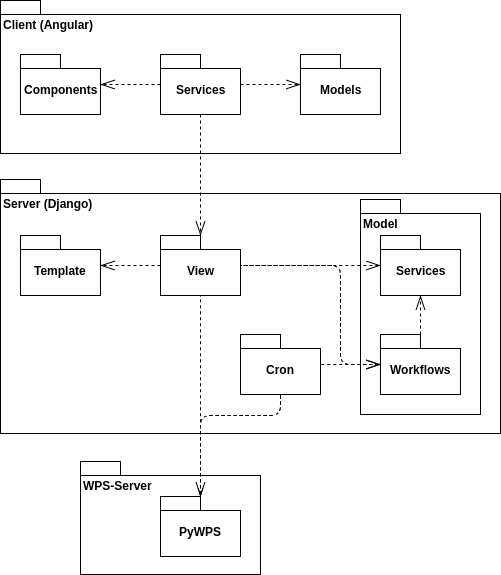
\includegraphics[scale=0.77]{images/package_diagram.png}
        \caption{Paketdiagramm}
        \label{fig:arch_package_division}
    \end{figure}
    
    \noindent Wie jede andere Web-Applikation, besteht das System aus Client- und Server-Teil, die miteinander mittels HTTP Requests kommunizieren.
    
        \subsection{Client-Teil}
        
        Der Client-Teil, der im Browser des Nutzers läuft ist auf dem JavaScript-Framework Angular aufgebaut. Es wurde aus folgenden Gründen ausgewählt:
        
        \begin{itemize}
            \item Idee: Angular ist ein Framework das für Anwendungen verwendet wird die meist direkt im Browser laufen, was bei WPSflow genau der Fall ist
            \item Angular bietet eine umfangreiche Funktionalität
            \item Eine hohe Qualität die durch eine große Community gewährleistet wird
            \item Es gibt eine vielzahl von Erweiterungen
            \item Die interne Benutzung von TypeScript, was ermöglicht streng typisierten Code zu schreiben und dadurch einige Fehler zu vermeiden und die Produktivität der Implementierung zu steigern
        \end{itemize}

        \noindent Angular-Apps sind nach MVC-Prinzip aufgebaut, wobei Views hier Components heißen und statt Controller man das Wort Services benutzt. Models repräsentieren die Datenstrukturen, Components sind für Anzeigen (Rendering) zuständig und Services handeln Ereignisse vom Benutzer, schicken Anfragen ans Client-Teil und empfängen Antworten davon.
        
        \subsection{Server-Teil}
        
        Auf dem Backend wird Python-Framework namens Django verwendet. Der benutzt ein wenig modifizierten MVC-Ansatz, der deswegen anderen Namen trägt - "Model - Template - View", kurz MTV.
        
        \begin{itemize}
            \item Model - definiert Datenstrukturen und dient dem Zugriff zur Datenbank
            \item View - "Controller" aus MVC 
            
            \begin{itemize}
                \item stellt zur Verfügung REST-Schnittstelle, die vom Client benutzt wird. Vorteil von solchem Ansatz ist, dass es wiederverwendbar ist, wenn man später nicht nur Web-Applikation haben will, sondern auch z. B. Smartphone-App
                \item handelt Abfragen vom Client, ruft Klassen aus dem Model-Paket, um Daten zu holen oder zu schreiben
            \end{itemize}
            \item Template - "View" aus MVC, enthält HTML der Seiten 
            \item Cron - wird in regelmäsigen Zeitabständen aufgerufen, fragt bei den WPS-Servern Status der momentan ausgeführten Tasks und, falls der Task erfolgreich beendet wurde, schickt ggf. nächsten Task auf den WPS-Server
        \end{itemize}
        
        \subsection{WPS-Server}
        
        Ein oder mehrere Server für eigentliche Berechnungen werden extern (nicht innerhalb unseres Projekts) zur Verfügung gestellt und in das System eingetragen, damit es darauf Abfragen schicken kann.
    